\subsection{Basic widgets and layouts}

\begin{frame}
  \frametitle{Basic examples -- widgets and layouts}
  \begin{itemize}
  \item Located in the \texttt{examples/02\_basic/} directory.
  \item Contains basic examples, introducing the following concepts.
    \begin{itemize}
    \item Commonly-used widgets.
    \item Commonly-used layouts.
    \end{itemize}
  \end{itemize}
\end{frame}

\subsection{Hello world - console}

\defverbatim[colored]\ExBasicLayoutsStructure{
\begin{lstlisting}[basicstyle=\scriptsize\ttfamily]
#include <QApplication>
// widgets
#include <QWidget>
#include <QPushButton>
#include <QLabel>
#include <QTextEdit>
#include <QCheckBox>
#include <QStatusBar>
// layout includes
// (*@\alert{include the layout header files here}@*)

int main(int argc, char *argv[])
{
	QApplication a(argc, argv);
	QWidget win;

	// (*@\alert{create the child widgets and layouts here}@*)

	win.show();

	return a.exec();
}\end{lstlisting}
}

\begin{frame}
  \frametitle{Basic structure of the examples -- common code}
  \ExBasicLayoutsStructure
\end{frame}

\defverbatim[colored]\ExBasicHVBoxLayoutsIncl{
\begin{lstlisting}[basicstyle=\tiny\ttfamily]
#include <QVBoxLayout>
#include <QHBoxLayout>
\end{lstlisting}
}

\defverbatim[colored]\ExBasicHVBoxLayoutsCode{
\begin{lstlisting}[basicstyle=\tiny\ttfamily]
QVBoxLayout* mainLayout = new QVBoxLayout();
// first row
QHBoxLayout* firstRowLayout = new QHBoxLayout();
firstRowLayout->addWidget(new QLabel("Label1", &win), 0);
firstRowLayout->addWidget(new QCheckBox("Flip me", &win), 2);
firstRowLayout->addWidget(new QPushButton("Push me", &win), 1);
mainLayout->addLayout(firstRowLayout, 0);
// second row
QHBoxLayout* secondRowLayout = new QHBoxLayout();
secondRowLayout->addWidget(new QLabel("Label2", &win), 0);
secondRowLayout->addWidget(new QTextEdit("Edit me", &win), 1);
mainLayout->addLayout(secondRowLayout, 0);
// button
QPushButton* clickButton = new QPushButton("Click me", &win);
mainLayout->addWidget(clickButton, 0, Qt::AlignCenter);
// status bar
QStatusBar* statusBar = new QStatusBar(&win);
statusBar->showMessage("Status text");
mainLayout->addWidget(statusBar, 0);

win.setLayout(mainLayout);
\end{lstlisting}
}

\begin{frame}
  \frametitle{Horizontal and vertical box layouts\footnote
    {\url{http://doc.qt.io/qt-5.6/qboxlayout.html}} -- code}
  \small
  Located in \texttt{examples/02\_basic/01\_hv\_layouts/}:
  \ExBasicHVBoxLayoutsIncl
  \ExBasicHVBoxLayoutsCode
\end{frame}

\begin{frame}
  \frametitle{Horizontal and vertical box layouts -- result}
  \begin{columns}
    \begin{column}{0.6\textwidth}
    \small
    This combination of \texttt{QHBoxLayout} and \texttt{QVBoxLayout}
    produces the following widget arrangement:
    \begin{figure}[!t]
    \centering
    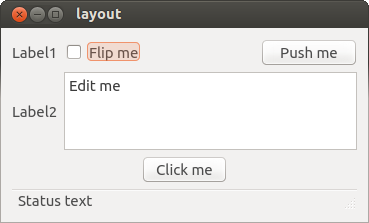
\includegraphics[width=\textwidth]{images/02_hv_layouts_wide.png}
    \end{figure}
    
    \end{column}
    \begin{column}{0.4\textwidth}
    \begin{figure}[!t]
    \centering
    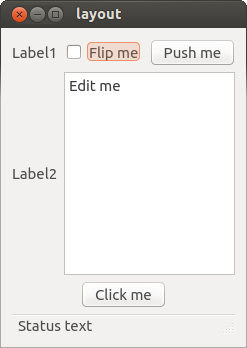
\includegraphics[width=\textwidth]{images/02_hv_layouts_tall.png}
    \end{figure}
    \end{column}
  \end{columns}
\end{frame}

\defverbatim[colored]\ExBasicFormLayoutIncl{
\begin{lstlisting}[basicstyle=\scriptsize\ttfamily]
#include <QFormLayout>
\end{lstlisting}
}

\defverbatim[colored]\ExBasicFormLayoutCode{
\begin{lstlisting}[basicstyle=\scriptsize\ttfamily]
QFormLayout* mainLayout = new QFormLayout();

mainLayout->addRow("Item1", new QLabel("Label", &win));
mainLayout->addRow("Item2", new QCheckBox("Checkbox",&win));
mainLayout->addRow("Item3", new QPushButton("Button",&win));
mainLayout->addRow("Item4", new QTextEdit("Text", &win));
mainLayout->addRow("Item5", new QSpinBox(&win));

win.setLayout(mainLayout);
\end{lstlisting}
}

\begin{frame}
  \frametitle{Form layout\footnote
    {\url{http://doc.qt.io/qt-5.6/qformlayout.html}} -- code}
  \small
  Located in \texttt{examples/02\_basic/02\_form\_layout/}:
  \ExBasicFormLayoutIncl
  \ExBasicFormLayoutCode
\end{frame}

\begin{frame}
  \frametitle{Form layout -- result}
  \begin{columns}
    \begin{column}{0.67\textwidth}
    \small
    \texttt{QFormLayout} produces the following widget arrangement:
    \begin{figure}[!t]
    \centering
    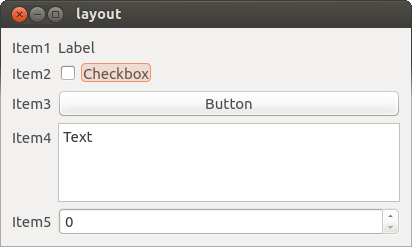
\includegraphics[width=\textwidth]{images/02_form_layout_wide.png}
    \end{figure}
    
    \end{column}
    \begin{column}{0.33\textwidth}
    \begin{figure}[!t]
    \centering
    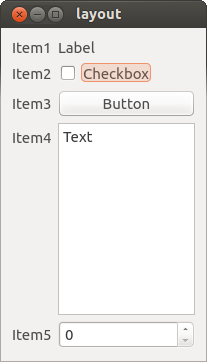
\includegraphics[width=\textwidth]{images/02_form_layout_tall.png}
    \end{figure}
    \end{column}
  \end{columns}
\end{frame}

\defverbatim[colored]\ExBasicGridLayoutIncl{
\begin{lstlisting}[basicstyle=\scriptsize\ttfamily]
#include <QGridLayout>
\end{lstlisting}
}

\defverbatim[colored]\ExBasicGridLayoutCode{
\begin{lstlisting}[basicstyle=\tiny\ttfamily]
QGridLayout* mainLayout = new QGridLayout();

mainLayout->addWidget(new QLabel("Label11", &win), 0,0);
mainLayout->addWidget(new QLabel("Label12", &win), 0,1);
mainLayout->addWidget(new QLabel("Label13", &win), 0,2);

mainLayout->addWidget(new QLabel("Label21", &win),       1,0);
mainLayout->addWidget(new QPushButton("Button22", &win), 1,1);
mainLayout->addWidget(new QCheckBox("CheckBox23", &win), 1,2);

mainLayout->addWidget(new QLabel("Label31", &win),       2,0);
mainLayout->addWidget(new QPushButton("Button32", &win), 2,1);
mainLayout->addWidget(new QTextEdit("Edit33", &win),     2,2);

mainLayout->setRowStretch(0, 0);
mainLayout->setRowStretch(1, 1);
mainLayout->setRowStretch(2, 2);

mainLayout->setColumnStretch(0, 0);
mainLayout->setColumnStretch(1, 1);
mainLayout->setColumnStretch(2, 2);
win.setLayout(mainLayout);
\end{lstlisting}
}

\begin{frame}
  \frametitle{Grid layout\footnote
    {\url{http://doc.qt.io/qt-5.6/qgridlayout.html}} -- code}
  \small
  Located in \texttt{examples/02\_basic/03\_grid\_layout/}:
  \ExBasicGridLayoutIncl
  \ExBasicGridLayoutCode
\end{frame}

\begin{frame}
  \frametitle{Grid layout -- result}
  \small
  \texttt{QGridLayout} produces the following widget arrangement:
  \begin{figure}[!t]
  \centering
  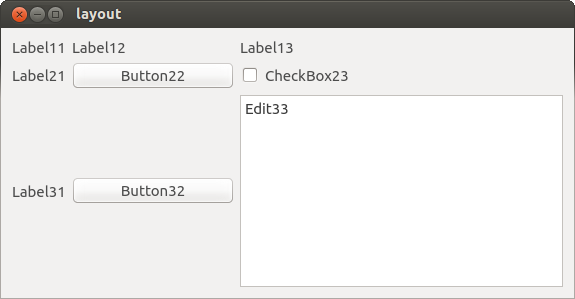
\includegraphics[width=0.85\textwidth]{images/02_grid_layout.png}
  \end{figure}
\end{frame}
